\section{Clasificador}

\subsection{Metodología}
\begin{frame}
    \frametitle{Metodología}

    \begin{itemize}
        \item Se utilizan SVM, kNN, DT, GNB y MNB.
        \item Se divide en 80\% entrenamiento y 20\% evaluación.
        \item Se usa validación cruzada sobre el conjunto de entrenamiento para resultados intermedios durante el desarollo y el conjunto de evaluación para el resultado final.
    \end{itemize}
\end{frame}
\note{
    Se explica a continuación qué es la validación cruzada.
    Se usa el conjunto de evaluación al final para no sesgarse demasiado a los resultados.
}

\subsubsection{Validación cruzada}
\begin{frame}
    \frametitle{Validación cruzada}
    
    \begin{center}
        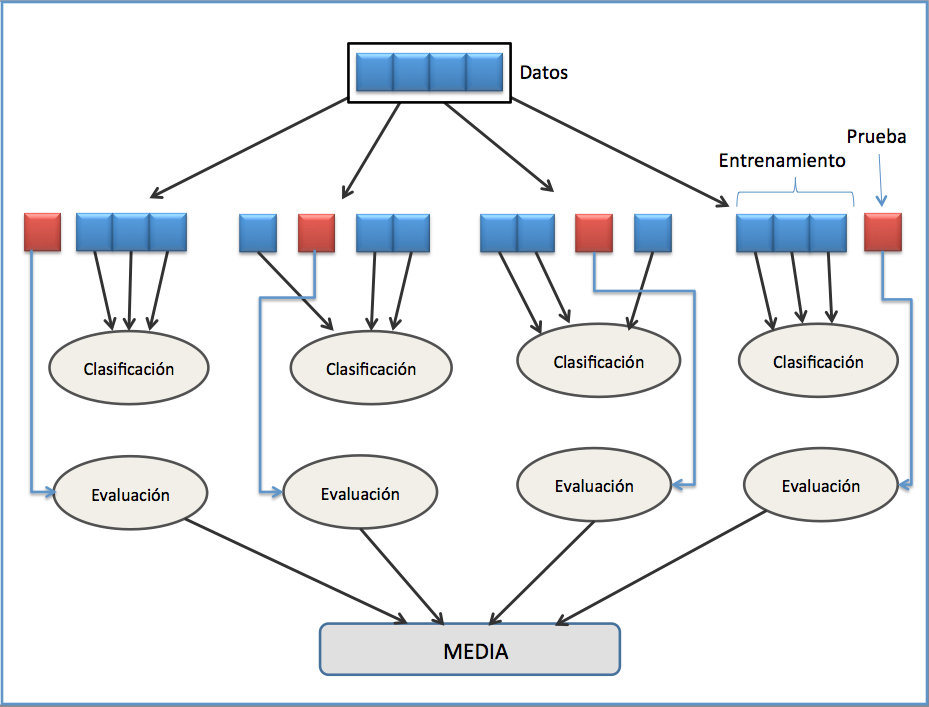
\includegraphics{cv.jpg}
    \end{center}
\end{frame}
\note{
    TODO: decir ventajas
}

% TODO: poner o no lo de subcorpus?

\subsection{Línea base}
\begin{frame}
    \frametitle{Línea base}

    \begin{enumerate}
        \item BoW + MNB
        \item Clasificador que predice según lo que dice la mayoría (No humor)
    \end{enumerate}
\end{frame}

\subsection{Características}

\begin{frame}
    \frametitle{Qué se busca}

    \begin{itemize}[<+->]
        \item Contradicción y negatividad
        \item Formato e informalidad
        \item Orientación en personas
        \item Temas recurrentes en chistes
    \end{itemize}
\end{frame}

\begin{frame}
    \frametitle{Presencia de animales}

    \begin{itemize}
        \item Se conforma una lista de animales a partir de los chistes de animales de Chistes.com ($DIC_A$)
        \item Intersección de multiconjuntos:
    \end{itemize}

    \begin{center}
        \[
            PresenciaAnimales(tweet) = \frac{|tweet \cap DIC_A|}{\sqrt{|tweet|}}
        \]
    \end{center}
\end{frame}
\note{
    Características simples.
    $tweet$ es visto como una lista de tokens.
    En general todas las featuers se normalizan según el largo del tweet en tokens, para no sesgar.
}

\begin{frame}
    \frametitle{Jerga sexual}

    \begin{itemize}
        \item Se arma un diccionario de jerga sexual mediante \emph{Bootstrapping} en Twitter.
        \item Intersección de multiconjuntos:
    \end{itemize}

    \begin{center}
        \[
            JergaSexual(tweet) = \frac{|tweet \cap DIC_{JS}|}{\sqrt{|tweet|}}
        \]
    \end{center}
\end{frame}

\begin{frame}
    \frametitle{Primera persona}

    \begin{itemize}
        \item Se busca por palabras flexionadas en primera persona
    \end{itemize}
\end{frame}

\begin{frame}
    \frametitle{Segunda persona}

    \begin{itemize}
        \item Se busca por palabras flexionadas en segunda persona
    \end{itemize}
\end{frame}

\begin{frame}
    \frametitle{Distancia temática}

    \begin{itemize}[<+->]
        \item Cercanía a un chiste de Chistes.com o cercanía a una oración de la Wikipedia.
        \item BoW + MNB
        \item Categorías
        \begin{itemize}[<+->]
            \item Chistes cortos
            \item Adivinanzas
            \item Animales
            \item Atlantes
            \item Otros...
        \end{itemize}
    \end{itemize}
\end{frame}

\begin{frame}
    \frametitle{Diálogo}

    \begin{itemize}
        \item Si el tweet es un diálogo o no
    \end{itemize}
\end{frame}

\begin{frame}
    \frametitle{Preguntas-respuestas}

    \begin{itemize}
        \item Cantidad de preguntas seguidas de respuestas en el tweet.
    \end{itemize}
\end{frame}

\begin{frame}
    \frametitle{Palabras frecuentes}

    \begin{itemize}
        \item Lista de palabras frecuentes en tweets
        \item Intersección de multiconjuntos:
    \end{itemize}

    \begin{center}
        \[
            PalabrasFrecuentes(tweet) = \frac{|tweet \cap DIC_{PF}|}{\sqrt{|tweet|}}
        \]
    \end{center}
\end{frame}

\begin{frame}
    \frametitle{Links}

    \begin{itemize}
        \item Cantidad de hipervínculos en el tweet
    \end{itemize}
\end{frame}

\begin{frame}
    \frametitle{Antónimos}

    \begin{itemize}
        \item Cantidad de pares de antónimos en el tweet:
    \end{itemize}

    \begin{center}
        \[
            Antonimos(tweet) = \frac{|\{pares de antonimos\}|}{\sqrt{|tweet|}}
        \]
    \end{center}
\end{frame}

\begin{frame}
    \frametitle{Hashtags}

    \begin{itemize}
        \item Cantidad de hashtags en el tweet
    \end{itemize}
\end{frame}

\begin{frame}
    \frametitle{Exclamación}

    \begin{itemize}
        \item Cantidad de signos de exclamación:
    \end{itemize}

    \begin{center}
        \[
            Exclamacion(tweet) = \frac{|\{signos de exclamacion\}|}{\sqrt{|tweet|}}
        \]
    \end{center}
\end{frame}

\begin{frame}
    \frametitle{Exclamación}

    \begin{itemize}
        \item Cantidad de palabras totalmente en mayúsculas:
    \end{itemize}

    \begin{center}
        \[
            PalabrasMayusculas(tweet) = \frac{|\{palabras mayusculas\}|}{\sqrt{|tweet|}}
        \]
    \end{center}
\end{frame}

\begin{frame}
    \frametitle{Negación}

    \begin{itemize}
        \item Cantidad de ``no'' en el tweet
    \end{itemize}
\end{frame}

\begin{frame}
    \frametitle{Palabras fuera del vocabluario}

    \begin{itemize}
        \item Cantidad de palabras fuera del vocabulario, dividiento entre el total
        \item Son varias características:
        \begin{itemize}
            \item Freeling
            \item Freeling-Google
            \item Freeling-Wiktionary
            \item Wiktionary
        \end{itemize}
    \end{itemize}
\end{frame}
\note{
    Las distintas combinaciones de vocabulario debido a costo de uso y debido a ventajas y desventajas de cada uno. \textbf{Freeling} el más barato de usar, offline. Tiene un español más clasico, pero no tiene palabras ``nuevas''. \textbf{Wiktionary} tiene un término medio de todo. Es online, pero no limita su uso. Con \textbf{Google} se pueden obtener muchas palabras ``nuevas'' (como iPhone) y también detección de errores ortográficos, pero limita su uso.
}

\begin{frame}
    \frametitle{Palabras no españolas}

    \begin{itemize}
        \item Cantidad de palabras que tienen caracteres fuera del alfabeto español, normalizado según el total.
    \end{itemize}
\end{frame}

\subsection{Primer clasificador}
\begin{frame}
    \frametitle{Primer clasificador}

    \begin{itemize}[<+->]
        \item Primero se optimizaron los parámetros de los distintos tipos de clasificadores
        \item Resultados

        \begin{center}
            \scriptsize
            \begin{tabular}{ c | r | r | r | r | r | r | r }
                \textbf{Clas./Med.} & precisión & recall & $F_1$ & prec. neg. & rec. neg. & $F_1$ neg. & acierto \\
                \hline
                \textbf{SVM} & \textbf{84,60} & 66,23 & \textbf{74,29} & 93,53 & 97,59 & \textbf{95,52} & \textbf{92,37} \\
                \hline
                \textbf{DT}  & 65,03 & 65,19 & 65,10 & 93,04 & 92,98 & 93,01 & 88,53 \\
                \hline
                \textbf{GNB} & 59,68 & \textbf{76,78} & 66,49 & \textbf{95,06} & 89,17 & 92,01 & 87,04 \\
                \hline
                \textbf{MNB} & 84,57 & 58,83 & 69,37 & 92,24 & \textbf{97,85} & 94,97 & 91,35 \\
                \hline
                \textbf{kNN} & 82,19 & 64,26 & 71,12 & 93,16 & 97,21 & 95,14 & 91,76 \\
            \end{tabular}
        \end{center}
    \end{itemize}
\end{frame}

\subsection{Selección de características}
\begin{frame}
    \frametitle{Selección de características}

    Selección de características
\end{frame}

\subsection{Clasificador final}
\begin{frame}
    \frametitle{Clasificador final}

    Clasificador final
\end{frame}

\subsection{Otros análisis}
\begin{frame}
    \frametitle{Otros análisis}

    Otros análisis
\end{frame}
